%
% Main document
% ===========================================================================
% This is part of the document "Project documentation template".
% Authors: brd3, kaa1
%

%---------------------------------------------------------------------------
\documentclass[
	a4paper,					% paper format
	10pt,							% fontsize
	twoside,					% double-sided
	notitlepage,			% use no standard title page
	parskip=half,			% set paragraph skip to half of a line
]{scrreprt}					% KOMA-script report
%---------------------------------------------------------------------------
\listfiles
\raggedbottom
\KOMAoptions{cleardoublepage=plain}			% Add header and footer on blank pages


% Load Standard Packages:
%---------------------------------------------------------------------------
\usepackage[standard-baselineskips]{cmbright}
\usepackage{svg}
\setsvg{inkscape=inkscape -z -D,svgpath=images/}
\usepackage{underscore}
\usepackage{transparent}
\usepackage{import}
\usepackage[ngerman]{babel}										% german hyphenation
\usepackage[utf8]{inputenc}  							% Unix/Linux - load extended character set (ISO 8859-1)
%\usepackage[ansinew]{inputenc}  							% Windows - load extended character set (ISO 8859-1)
\usepackage[T1]{fontenc}											% hyphenation of words with ä,ö and ü
\usepackage{textcomp}													% additional symbols
\usepackage{ae}																% better resolution of Type1-Fonts
\usepackage{fancyhdr}													% simple manipulation of header and footer
\usepackage{etoolbox}													% color manipulation of header and footer
\usepackage{graphicx}                      		% integration of images
\usepackage{float}														% floating objects
\usepackage{caption}													% for captions of figures and tables
\usepackage{booktabs}													% package for nicer tables
\usepackage{tocvsec2}													% provides means of controlling the sectional numbering
\usepackage{listings}
\usepackage{tabularx}

\usepackage{listings}

\usepackage{pdflscape}
%\usepackage{lscape}
%---------------------------------------------------------------------------

% Load Math Packages
%---------------------------------------------------------------------------
\usepackage{amsmath}                    	   	% various features to facilitate writing math formulas
\usepackage{amsthm}                       	 	% enhanced version of latex's newtheorem
\usepackage{amsfonts}                      		% set of miscellaneous TeX fonts that augment the standard CM
\usepackage{amssymb}													% mathematical special characters
\usepackage{exscale}													% mathematical size corresponds to textsize
%---------------------------------------------------------------------------

% Package to facilitate placement of boxes at absolute positions
%---------------------------------------------------------------------------
\usepackage[absolute]{textpos}
\setlength{\TPHorizModule}{1mm}
\setlength{\TPVertModule}{1mm}
%---------------------------------------------------------------------------

% Definition of Colors
%---------------------------------------------------------------------------
\RequirePackage{color}                          % Color (not xcolor!)
\definecolor{linkblue}{rgb}{0,0,0.8}            % Standard
\definecolor{darkblue}{rgb}{0,0.08,0.45}        % Dark blue
\definecolor{bfhgrey}{rgb}{0.41,0.49,0.57}      % BFH grey
%\definecolor{linkcolor}{rgb}{0,0,0.8}     			% Blue for the web- and cd-version!
\definecolor{linkcolor}{rgb}{0,0,0}        			% Black for the print-version!
%---------------------------------------------------------------------------

% Hyperref Package (Create links in a pdf)
%---------------------------------------------------------------------------
\usepackage[
	pdftex,english,bookmarks,plainpages=false,pdfpagelabels,
	backref = {false},										% No index backreference
	colorlinks = {true},                  % Color links in a PDF
	hypertexnames = {true},               % no failures "same page(i)"
	bookmarksopen = {true},               % opens the bar on the left side
	bookmarksopenlevel = {0},             % depth of opened bookmarks
  pdftitle = {{Presentator3000, an online presentation tool}},	   	% PDF-property
  pdfauthor = {{bollm6, schmr2}},        					  % PDF-property
	pdfsubject = {Presentator3000},        % PDF-property
	linkcolor = {linkcolor},              % Color of Links
	citecolor = {linkcolor},              % Color of Cite-Links
	urlcolor = {linkcolor},               % Color of URLs
]{hyperref}
%---------------------------------------------------------------------------

% Set up page dimension
%---------------------------------------------------------------------------
\usepackage{geometry}
\geometry{
	a4paper,
	left=28mm,
	right=15mm,
	top=30mm,
	headheight=20mm,
	headsep=10mm,
	textheight=242mm,
	footskip=15mm
}
%---------------------------------------------------------------------------

% Makeindex Package
%---------------------------------------------------------------------------
\usepackage{makeidx}                         		% To produce index
\makeindex                                    	% Index-Initialisation
%---------------------------------------------------------------------------

% Intro:
%---------------------------------------------------------------------------
\begin{document}                              	% Start Document
\settocdepth{section}														% Set depth of toc
\pagenumbering{roman}
%---------------------------------------------------------------------------
\providecommand{\titel}{Presentator3000}		%  Hier den Titel des Berichts/Thesis eingeben
\providecommand{\versionnumber}{1.0}			%  Hier die aktuelle Versionsnummer eingeben
\providecommand{\versiondate}{2016-11-13}		%  Hier das Datum der aktuellen Version eingeben

% Set up header and footer
%---------------------------------------------------------------------------
\makeatletter
\patchcmd{\@fancyhead}{\rlap}{\color{bfhgrey}\rlap}{}{}		% new color of header
\patchcmd{\@fancyfoot}{\rlap}{\color{bfhgrey}\rlap}{}{}		% new color of footer
\makeatother

\fancyhf{}																		% clean all fields
\fancypagestyle{plain}{												% new definition of plain style
	\fancyfoot[OR,EL]{\footnotesize \thepage} 	% footer right part --> page number
	\fancyfoot[OL,ER]{\footnotesize \titel, Version \versionnumber, \versiondate}	% footer even page left part
}

\renewcommand{\chaptermark}[1]{\markboth{\thechapter.  #1}{}}
\renewcommand{\headrulewidth}{0pt}				% no header stripline
\renewcommand{\footrulewidth}{0pt} 				% no bottom stripline

\pagestyle{plain}
%---------------------------------------------------------------------------


% Title Page and Abstract
%---------------------------------------------------------------------------
%
% Project documentation template
% ===========================================================================
% This is part of the document "Project documentation template".
% Authors: brd3, kaa1
%

\begin{titlepage}

\graphicspath{{./images/}}


% BFH-Logo absolute placed at (28,12) on A4 and picture (16:9 or 15cm x 8.5cm)
% Actually not a realy satisfactory solution but working.
%---------------------------------------------------------------------------
\setlength{\unitlength}{1mm}
\begin{textblock}{20}[0,0](28,12)
	\includegraphics[scale=1.0]{\detokenize{BFH_Logo_B.png}}
\end{textblock}

\begin{textblock}{154}(28,48)
	\begin{picture}(150,2)
		\put(0,0){\color{bfhgrey}\rule{150mm}{2mm}}
	\end{picture}
\end{textblock}

\begin{textblock}{154}[0,0](28,50)
	
\includegraphics[width=15cm]{images/head}			% Titelbild definieren
\end{textblock}

\begin{textblock}{154}(28,162)
	\begin{picture}(150,2)
		\put(0,0){\color{bfhgrey}\rule{150mm}{2mm}}
	\end{picture}
\end{textblock}
\color{black}

% Institution / Titel / Untertitel / Autoren / Experten:
%---------------------------------------------------------------------------
\begin{flushleft}

\vspace*{130mm}

\fontsize{26pt}{28pt}\selectfont
\titel 				\\							% Titel aus der Datei vorspann/titel.tex lesen
\vspace{2mm}

\fontsize{16pt}{20pt}\selectfont\vspace{0.3em}
\vspace{5mm}

\fontsize{10pt}{12pt}\selectfont
\textbf{Projektdokumentation} \\									% eingeben
\vspace{3mm}

% Abstract (eingeben):
%---------------------------------------------------------------------------
\begin{textblock}{150}(28,190)
\fontsize{10pt}{12pt}\selectfont
Diese Dokumentation berschreibt die geleistete Arbeit im Rahmen des Projekt 2. \\
\end{textblock}

\begin{textblock}{150}(28,225)
\fontsize{10pt}{17pt}\selectfont
\begin{tabbing}
xxxxxxxxxxxxxxx\=xxxxxxxxxxxxxxxxxxxxxxxxxxxxxxxxxxxxxxxxxxxxxxx \kill
Studiengang:	\> Informatik	\\			% Namen eingeben
Kurs:        \> Project 2 \\
Autoren:        \> Michael Bolli (michael.bolli.1@students.bfh.ch), \\
\>Robin Schmid (robinsamuel.schmid@students.bfh.ch)		\\					% Namen eingeben
Betreuung:	    \> Marcel Pfahrer		\\					% Namen eingeben
Datum:			\> 03.02.2017				\\		% aus Datei vorspann/version.tex lesen
\end{tabbing}

\end{textblock}
\end{flushleft}

\begin{textblock}{150}(28,280)
\noindent
\color{bfhgrey}\fontsize{9pt}{10pt}\selectfont
Berner Fachhochschule | Haute école spécialisée bernoise | Bern University of Applied Sciences
\color{black}\selectfont
\end{textblock}


\end{titlepage}

\setcounter{page}{1}
\tableofcontents

%---------------------------------------------------------------------------

%w--------------------------------------------------------
\pagenumbering{arabic}
\color{black}

\chapter{Einführung}
\label{chap:intro}

\section{Ausgangslage}
Wenn heute an der Berner Fachhochschule oder anderen Einrichtungen Vorlesungen abgehalten werden, kommen häufig Bildschirmpräsentationen zum Einsatz. Diese unterstützen das Erzählte und helfen den Dozenten, einen roten Faden zu ziehen. Weiter können die Folien (nachfolgend auch Slides genannt) den Unterrichteten abgegeben werden. Diese wiederum können die Unterlagen verwenden, um den Stoff zu repetieren und sich für Examen vorzubereiten. Solche Bildschirmpräsentationen können auf diverse Arten erstellt werden. Die bekannteste Möglichkeit stellt wohl Microsofts PowerPoint dar. Diese Software ist nicht nur sehr anwenderfreundlich sondern auch weit verbreitet. Doch nebst den Anschafungskosten ist PowerPoint abhängig vom Betriebssystem. Für Linux und Unix Systeme (ausser OSX) existiert das Produkt nicht. Gerade in wissenschaftlichen Kreisen verwendet jedoch ein stattlicher Prozentsatz andere Betriebssysteme als Windows/OSX. Als Alternative kommen diverse Varianten zum Einsatz: LibreOffice, OpenOffice, PDFs (aus Latex Vorlagen oder auch andere Quellen), etc. Mit dem aufkommen von Breitband-Internet gibt es auch immer mehr plattformunabhänige Tools, welche direkt im Browser funktionieren. Beispiele dafür sind\emph{Google Slides} oder \emph{Prezi}. 

Nun kommt im spezifischen Fall der BFH TI noch ein weitere Anwendungsfall hinzu: Das Präsentieren von Programmiercode. Dieser Code oder Code-Ausschnitt (nachfolgend auch Code-Fragment, Snippet genannt) ist meist Teil eines grösseren Gesamtkontexts wie etwa einer Übung oder eines Beispiels. Diese Unterlagen werden von den Dozierenden laufend verändert und optimiert. So müssen auch die Präsentationen angepasst werden. Um hier eine Dynamisierung zu schaffen, müsste der Code flexibel in die Präsentation eingebunden werden. Dieser Grundgedanke führte zur Idee eines neuen Produktes, welches nachfolgend erklärt wird.

\section{Idee}
Das Leitmotiv besteht daraus, eine Applikation zu erstellen, welche von Dozenten und Schülern gleichermassen verwendet werden kann. Im Zentrum steht dabei das einfache Erstellen und teilen von Bildschirmpräsentationen. Hinzu kommt das Hinzufügen und Verwalten von Code-Fragmenten. Programmiercode, welcher in einem Repository verfügbar ist, soll auf einfache Weise zu einer Slide hinzugefügt werden können. Wird ein Teil des Snippets geändert, soll die Präsentation mit einer einfachen Aktion (Klick) aktualisiert werden können. Somit gehört das manuelle Anpassen von Code in Präsentationen der Vergangenheit an. 

Um den verschiedenen Geräten und Betriebssystem potenzieller Nutzer Herr zu werden, soll die Applikation als Web-App in gängigen Web-Browsern nutzbar sein.

Eine weitere Funktionalität ist das das Kommentieren von Slides. Hat ein Schüler eine Frage zu einem behandelten Punkt in einem Slide, kann er einen Kommentar hinzufügen. Der Dozierende oder auch Kommilitonen können dann antworten und ihm weiterhelfen. Natürlich kann die Kommentarfunktion auch dazu verwendet werden, um auf Fehler hinzuweisen oder anderen Benutzern weitere Informationen zu verlinken.

Slides sollen nicht fix einer Präsentation angehören, sondern nach Bedarf in eine Präsentation eingefügt werden können. Somit sind Slides wiederverwendbare Komponenten. Um den Überblick an erstellten Slides und Präsentationen zu behalten, lassen sich beide durch das hinzufügen von Tags thematisch kategorisieren. Des weiteren sollen Nutzer sogenannte \emph{Channels} erstellen können, wo sie ihre Präsentationen hinzufügen können. Ein \emph{Channel} dient dazu, anderen Nutzer, beispielsweise Studenten eines Kurses, alle relevanten Präsentationen dieses Kurs geordnet darzustellen. Abonnenten (\emph{Subscriber}) eines \emph{Channels} werden dann benachrichtigt, sobald eine neue Präsentation verfügbar ist oder sich etwas an einer bestehenden Präsentation geändert hat. 

Um die Darstellung von Slides zu beeinflussen sind zwei Funktionen geplant: Mit \emph{Templates} soll eine gewisse Grundstruktur vorgegeben werden. Diese kann in den Editor übernommen und dort bearbeitet werden. Es gibt Templates für Titelfolien, Inhaltsfolien, usw. Die Applikation selbst kommt bereits mit einer Grundmenge an Templates und der User soll nach Bedarf selbst neue hinzufügen können. Um die Gestaltung sind sogenannte \emph{Themes} zuständig. Sie steuern mit CSS-Ausdrücken das Layout einer Präsentation. Auch hier gibt es bereits vorgefertigte Vorlagen, aber auch die Möglichkeit für den User, eigene zu erstellen.

Um den Zuschauern die bestmögliche Erfahrung zu bieten, sollen Präsentationen auch gedruckt beziehungsweise als PDF heruntergeladen werden können. Auch sollen Zuschauer eine Präsentation mit einem spezifischen Link in ihrem eigenen Webbrowser aufrufen können. Dies dient dazu, in überfüllten Hörsälen den Gästen in den hintersten Reihen trotzdem eine optimale Sicht auf die Geschehnisse auf dem Bildschirm zu bieten.

Die aufgezählten Features sind nicht für jeden Benutzer in gleicher Ausführung verfügbar. Je nach Ausgestaltung  des Geschäftsmodel können gewisse Funktionen gar nicht oder nur in limitierter Ausprägung verwendet werden. Es ist aber auch denkbar, das für die Quantität (pro Slide, pro Präsentation, pro Theme, pro Template) eine Microtransaction gestellt wird. Die geeignetste Art der Monetariserung muss in der Entwicklung des Projekts evaluiert werden.



\chapter{Anforderungen}
\label{chap:requirements}

\section{Ziel}
\label{sec:ziel}

\subsection{Hauptziel}
Das Ziel ist es, eine Applikation zu entwickeln, welche die Erstellung und das Vorführen von Präsentationen ermöglicht. Die Funktionalitäten sollen "as a service" im Browser angeboten werden.

\begingroup
\setlength{\tabcolsep}{10pt} % Default value: 6pt
\renewcommand{\arraystretch}{1.5}
\subsection{Unterziele}
\begin{tabularx}{\textwidth}{ |l|X| }
  \hline
  \textbf{Z 1}	& \textbf{Wirtschaftliche Ziele}	\\	\hline
  Z 1.1	& Der Entwicklungsaufwand für die Umsetzung eines System ist bekannt.  	\\	\hline
  Z 1.2	& Die Betriebskosten für ein umgesetztes System mit Skalierung ist bekannt.  	\\	\hline
  Z 1.3	& Es liegt eine Beurteilung des Marktpotentials vor.  	\\	\hline
  Z 1.4	& Es wurde ein Konzept zur Monetarisierung (Geschäftsmodell) entwickelt. 	\\	\hline
  \hline
  \textbf{Z 2}	& \textbf{Technische Ziele}	\\	\hline
  Z 2.1	& Die Eignung möglicher Frameworks und Technologien für die Umsetzung des Backends wurde geprüft und ein Typenentscheid gefällt.	\\	\hline
  Z 2.2	& Die Eignung möglicher Frameworks und Technologien für die Umsetzung des Frontends wurde geprüft und ein Typenentscheid gefällt.	\\	\hline  
  Z 2.3	& Es existiert eine Umsetzung der Applikation, welche die Prognose zur Weiterentwicklung unterstützt (Prove of Concept) \\	\hline    
  Z 2.4	& Es ist eine Schnittstelle zwischen Frontend und Backend definiert, um die Kommunikation zwischen den Applikationsteilen zu vereinheitlichen. \\	\hline   
  \end{tabularx}
\endgroup


\section{Systemkontext}
\label{sec:systemkontext}
Der Systemkontext umfasst mehrere Teilbereiche. Der Anwender sieht jeweils nur das Frontend, welches als Single-Page-Application ausgeliefert wird. Die Kopplung zur Datenverwaltung im Backend (Server) ist sehr lose. Dies erlaubt, nach Bedarf Teile des Systems neu zu entwickeln oder Technologien zu ersetzen, wenn diese Veraltet sind, ohne das ganze System neu zu bauen. 

Die Darstellung (View) wird als Webinterface an den Webbrowser des Benutzers ausgeliefert. Er benötigt somit keine zusätzliche Software. Die Ausgabe des Frontend hängt von der Verwendung ab und kann auf einem Monitor, Beamer oder auch Smartphone erfolgen. Wird beispielsweise eine Präsentation vorgeführt, muss sie auf einem Projektor oder einem grossen Bildschirm dargestellt werden. Der Nutzer will aber gleichzeitig die Präsentation steuern und kann auf seinem Smartphone Notizen zur aktuellen Folie einsehen. Er kann dafür aber auch seinen Laptop verwenden. Das Layout soll deshalb \textbf{responsive} sein. Da das Gerät des Users dem System nicht zum Voraus bekannt ist, kann die Darstellung (View) keine systembezogenen Funktionalitäten voraussetzen, sprich muss mit einer grossen Anzahl von Browsern kompatibel sein.

Das Backend soll wie bereits erwähnt technologisch möglichst unabhängig von der Darstellung sein. Es muss zudem auf einem System zu laufen kommen, welches auf Geschwindigkeit optimiert ist. Daten sollen schnell geschrieben und gelesen werden. 

\section{Anforderungen}
\label{sec:anforderungen}

\subsection{Einführung}
Im folgenden Kapitel werden die Anfordungen, die sich für das Projekt ergeben, dokumentiert. In der Detailbeschreibung wurde die natürlichsprachige Form gewählt.

\subsubsection{Legende und ergänzende Hinweise}

\minisec{Priorität (P)}
Die Prioritäten sind wie folgt gegliedert:
\begin{itemize}
	\item 0: Optional
	\item 1: Niedrige Priorität
	\item 2: Mittlere Priorität
	\item 3: Hohe Priorität
\end{itemize}

\minisec{Variabilität (V)}
\begin{itemize}
	\item 1: Niedrige Variabilität
	\item 2: Mittlere Variabilität
	\item 3: Hohe Variabilität
\end{itemize}

\minisec{Komplexität (K)}
\begin{itemize}
	\item 1: Niedrige Komplexität
	\item 2: Mittlere Komplexität
	\item 3: Hohe Komplexität
\end{itemize}

\minisec{Risiko (R)}
Aus den drei Faktoren Priorität, Variabilität und Komplexität wurde das Risiko im gesamten Projektrahmen errechnet. Die Faktoren wurden unterschiedliche gewichtet, Komplexität am höchsten und Priorität am tiefsten. 

\minisec{Ergänzungen}
Unter Quelle ist jeweils ersichtlich, woher die Anforderung stammt. Folgende Abkürzungen werden verwendet:
\begin{itemize}
	\item RE: Requirement Engineering
	\item M: Meeting
	\item B: Betreuer
\end{itemize}
In der tabellarischen Form ist jeweils in der Spalte \emph{Ziel} ersichtlich, auf welches Unterziel sich die Anforderung bezieht. Es ist auch möglich, dass sich die Anforderung direkt auf das Hauptziel bezieht; in diesem Fall ist \emph{HZ} notiert.

\subsection{Funktionale Anforderungen}
\subsubsection{Übersicht}
\begingroup
\setlength{\tabcolsep}{10pt} % Default value: 6pt
\renewcommand{\arraystretch}{1.1}
\begin{tabularx}{\textwidth}{ |l|X|c|c|c|c|c|c| }
  \hline
	Nr.	&	Kurzbeschrieb	& 	P	& 	V	&	K	&	R	&	Quelle	&	Ziel	\\	\hline
	R 1	&	Das System ermöglicht es Nutzern, sich zu registrieren &	3	&	1	&	1	& 	1	&	RE	&	HZ	\\	\hline
	R 2	&	Das System ermöglicht es dem Nutzer, Präsentationen zu erstellen &	3	&	2	&	3	& 	3	&	C	&	Z 2.3	\\	\hline
	R 3	&	Das System ermöglicht es dem Nutzer, Slides zu erstellen und einer Präsentation hinzuzufügen &	3	&	1	&	2	&	2	&	M	&	HZ	\\ \hline
	R 4	&	Das System ermöglicht es dem Nutzer, Vorlagen (Templates) für Slides zu erstellen und diese beim erstellen von neuen Slides zu verwenden		&	1	&	2	& 	3	&	3	&	M	&	HZ	\\ \hline
	R 5	&	Das System ermöglicht es dem Nutzer, Themas (Themes) zu erstellen	&	0	& 	1	&	3	& 	0	&	C	&	? \\ \hline
	R 6	&	Das System ermöglicht es dem Nutzer, erstellte Präsentationen per Webbrowser zu präsentieren	&	3	& 	1	&	3	& 	0	&	C	&	HZ \\ \hline
	R 7	&	Das System ermöglicht es dem Nutzer, erstellte Präsentationen mit anderen Benutzer zu teilen	&	1	& 	1	&	2	& 	0	&	C	&	HZ \\ \hline
	R 8	&	Das System ermöglicht es dem Nutzer, Beilagen zu Präsentationen hinzuzufügen	&	1	& 	1	&	2	& 	0	&	RE	&	HZ \\ \hline
	R 9	&	Das System ermöglicht es dem Nutzer, Präsentationen in Channels zu organisieren	&	1	& 	1	&	2	& 	0	&	RE	&	HZ \\ \hline
\end{tabularx}
\endgroup

\subsection{Qualitätsanforderungen}

\subsubsection{Übersicht}
\begingroup
\setlength{\tabcolsep}{10pt} % Default value: 6pt
\renewcommand{\arraystretch}{1.5}
\begin{tabularx}{\textwidth}{ |l|X|c|c|c|c|c|c| }
  \hline
	Nr.	&	Kurzbeschrieb	& 	P	& 	V	&	K	&	R	&	Quelle	&	Ziel \\	\hline
	Q 1	&	Bei der Vorführung einer Präsentation beträgt die Latenz zwischen Eingabe und Ausgabe weniger als 30 ms	&	2	&	1	&	2	& 	2	&	RE	&	?	\\	\hline
\end{tabularx}
\endgroup
\chapter{Technologien}
\label{chap:techstack}

\section{Frontend}
Für die Entwicklung moderner Webanwendungen stehen viele Verschiedene Boilerplates, Libraries und Frameworks zu Verfügung. Deshalb ist es sinnvoll, sich mit den Technologien auseinander zu setzen und sich schliesslich für eine Variante zu entscheiden. Um bei der Entwicklung der Applikation effizient zu sein, ist es nötig, diejenigen Technologien auszuwählen, die das Schreiben von Code minimieren und schnell erlernbar sind. Für eine moderne Web-App werden deshalb häufig Frameworks gegenüber purem JavaScript oder JQuery bevorzugt. Solche Frameworks sind dazu ausgelegt, mit API zu kommunizieren und erhaltene Daten aufzubereiten und darzustellen. Hier eine Auswahl:

\begin{itemize}
	\item \textbf{AngularJS}
	\item \textbf{Backbone.js}
	\item \textbf{Knockout.js}
	\item \textbf{Vue.js}
\end{itemize}

Von den oben genannten ist uns bei der Evaluierung \emph{Vue.js} ins Auge gestochen. Nach Betrachtung der Dokumentation und Gesprächen mit Entwicklerkollegen, die \emph{vue} bereits verwendet haben, konnten wir uns darauf festlegen. \emph{Vue.js} ist ein Framework, welches das MVVM Entwurfsmuster umsetzt und ist gemäss Angaben der Entwickler einfacher zu erlernen als andere ähnliche Frameworks.

Für die Darstellung der Präsentation wurde \emph{reveal.js} ausgewählt. Es handelt sich hierbei um ein Framework, welches die Erstellung und Animation von HTML-Präsentationen erleichtert. 

Um den eingebetteten Code auf den Slides mit Syntax-Highlighting lesbarer zu machen, wurde eine Library names \emph{highlight.js} ausgewählt. Eine Alternative dazu wäre \emph{Prism JS} gewesen. 


\section{Backend}

Um die Datenpersistenz sicher und stabil zu machen, wird häufig auch im Backend ein Framework eingesetzt. Hier hängt der Entschluss vor allem vom verwendeten Betriebssystem und der präferierten Programmiersprache ab. Es wurde in erster Linie darauf geachtet, dass die Applikation möglichst einfach auf ein Produktionssystem aufgespielt werden kann. Es bietet sich PHP als Programmiersprache an, da diese auf den meisten Webservern schon installiert ist. Auch hier gibt es diverse Frameworks. Der Entscheid fiel auf Laravel, da es einfach zu erlernen ist und das Wissen momentan in Fachkreisen sehr gefragt ist. Laravel kann mit verschiedenen Datenbanken zusammen verwendet werden. Schliesslich wurde MySQL verwendet, da auch dies schon auf vielen Webservern vorhanden ist, was wiederum die Einrichtung eines produktiven System erleichtert. 
\chapter{Domain Model}
\label{chap:domainmodel}

\begingroup
\setlength{\tabcolsep}{15pt} % Default value: 6pt
\renewcommand{\arraystretch}{1.2}
\begin{table}[h]
\centering
\begin{tabular}{l|c|c|c}
	\textbf{Features} 	&	\textbf{Silver} 	&	\textbf{Gold}	&	\textbf{Diamond} \\ \hline
	Anzahl Präsentationen	&	10	&	unlimitiert	&	unlimitiert \\ \hline
	Anzahl Slides pro Präsentation	&	30	&	unlimitiert	& unlimitiert \\ \hline
	Anzahl Codebases	&	1	& 	unlimitiert	&	unlimitiert \\ \hline
	Channels		&	Nein	&	Nein	& 	Ja, unlimitiert	\\ \hline
	Attachements		&	Nein	&	Nein	&	Ja, unlimitiert \\ \hline
	Preis	&	\textbf{Gratis}	&	\textbf{CHF 5 / Monat} 	& \textbf{CHF 20 / Monat}
\end{tabular}
\end{table}
\endgroup

\begin{figure}[htbp]
    \includesvg[width = 1\textwidth,pdf,path=images/]{erm}
    \caption{Domain Model}
\end{figure}
\chapter{Use Cases}
\label{usecases}

\section{Use Case Diagramm}

\section{Use Case Beschreibungen}
\label{usecase:description}

\subsection{UC 001: Register}
\label{uc:001-register}
\begin{tabular}{|l|p{0.6\textwidth}|}
\hline
\textbf{Use Case Name} 	&	Register	\\ \hline
\textbf{Primary Actor} 	&		\\ \hline
\textbf{Stakeholders}	&		\\ \hline
\textbf{Preconditions}	&		\\ \hline
\textbf{Main Success Scenario}	& 	
\begin{enumerate}
	\item Der EnterpriseManager gibt eine valide Emailadresse und zweimal ein sicheres Passwort ein.
\end{enumerate}
\\ \hline
\textbf{Extensions}	&
\\ \hline
\end{tabular}

\subsection{UC 002: Login}
\label{uc:002-login}

\begin{tabular}{|l|p{0.6\textwidth}|}
\hline
\textbf{Use Case Name} 	&	Login	\\ \hline
\textbf{Primary Actor} 	&	User	\\ \hline
\textbf{Stakeholders}	&	-	\\ \hline
\textbf{Preconditions}	&	Der User ist im System registriert (\nameref{uc:001-register}) und hat seinen Account aktiviert.	\\ \hline
\textbf{Main Success Scenario}	& 	
\begin{enumerate}
	\item Der User gibt seine E-Mail-Adresse und sein Passwort ein
	\item Das System überprüft ob ein Account mit dieser E-Mail Adresse besteht
	\item Das System überprüft, ob das Passwort mit dem des Accounts übereinstimmt
	\item Das System überprüft, ob der Account bereits aktiviert wurde
	\item Der User wird in das System eingeloggt
\end{enumerate}
\\ \hline
\textbf{Extensions}	& 	
\begin{enumerate}
\setcounter{enumi}{1}
    \item
    \begin{enumerate}
    \item Es existiert kein Account mit der eingegebenen E-Mail-Adresse: Das System macht den User darauf aufmerksam
    \end{enumerate}
    \item
    \begin{enumerate}
    \item Das eingegebene Passwort stimmt nicht mit dem Passwort des Accounts überein: Der User wird darauf hingewiesen, dass das Passwort falsch ist und er kann es noch einmal eingeben
    \end{enumerate}
    \item
    \begin{enumerate}
    \item Der Account ist noch nicht aktiviert, was bedeutet, der User hat den Aktivierungslink noch nicht verwendet: Dem User wird angeboten, den Aktivierungslink noch einmal zu versenden
    \end{enumerate}
\end{enumerate}
\\ \hline
\end{tabular}

\subsection{UC 003: Logout}
\label{uc:003-logout}

\begin{tabular}{|l|p{0.6\textwidth}|}
\hline
\textbf{Use Case Name} 	&	Logout	\\ \hline
\textbf{Primary Actor} 	&		\\ \hline
\textbf{Stakeholders}	&		\\ \hline
\textbf{Preconditions}	&	Der User ist im System eingeloggt.(\nameref{uc:002-login}).	\\ \hline
\textbf{Main Success Scenario}	& 	
\begin{enumerate}
	\item Der User wählt die Schaltfläche \emph{Ausloggen} aus
	\item Das System loggt den User aus.
\end{enumerate}
\\ \hline
\textbf{Extensions}	& 	\\ \hline
\end{tabular}

\subsection{UC 004: Manage Presentation}
\label{uc:004-manage-pres}

\begin{tabular}{|l|p{0.6\textwidth}|}
\hline
\textbf{Use Case Name} 	&	Manage Presentation	\\ \hline
\textbf{Primary Actor} 	&		\\ \hline
\textbf{Stakeholders}	&		\\ \hline
\textbf{Preconditions}	&	Anzahl bestehender Präsentationen ist kleiner gleich max_presentations des Abo-Plans.	\\ \hline
\textbf{Main Success Scenario}	&
\begin{enumerate}
	\item Ein eingeloggter User kann Präsentationen hinzufügen
	\item Eine Präsentation besteht aus Slides in einer definierten Reihenfolge
	\item Eine Präsentation ist in der Grösse durch max_slides_pp des Abo-Plans beschränkt.
\end{enumerate}
\\ \hline
\textbf{Extensions}	& 	\\ \hline
\end{tabular}

\subsection{UC 005: Manage Slide}
\label{uc:005-manage-slide}

\begin{tabular}{|l|p{0.6\textwidth}|}
\hline
\textbf{Use Case Name} 	&	Manage Slide	\\ \hline
\textbf{Primary Actor} 	&		\\ \hline
\textbf{Stakeholders}	&		\\ \hline
\textbf{Preconditions}	&	Anzahl Slides in einer Präsentation ist kleiner gleich max_slides_pp des Abo-Plans.	\\ \hline
\textbf{Main Success Scenario}	&
\begin{enumerate}
	\item Ein eingeloggter User kann einer Präsentation Slides hinzufügen
	\item Ein Slide kann in einer anderen Präsentation wiederverwendet werden (shared = true)
	\item Ein Slide kann mithilfe eines WYSIWYG-Editors benutzerfreundlich bearbeitet werden
	\item Slides können in der Reihenfolge via Drag'n'Drop angepasst werden
\end{enumerate}
\\ \hline
\textbf{Extensions}	& 	\\ \hline
\end{tabular}

\subsection{UC 006: Share Presentation}
\label{uc:006-share-pres}

\subsection{UC 007: View Presentation}
\label{uc:007-view-pres}

\begin{tabular}{|l|p{0.6\textwidth}|}
\hline
\textbf{Use Case Name} 	&	View Presentation	\\ \hline
\textbf{Primary Actor} 	&		\\ \hline
\textbf{Stakeholders}	&		\\ \hline
\textbf{Preconditions}	&		\\ \hline
\textbf{Main Success Scenario}	&
\begin{enumerate}
	\item Die Präsentation wird angezeigt
\end{enumerate}
\\ \hline
\textbf{Extensions}	& 	\\ \hline
\end{tabular}

\subsection{UC 008: Print Presentation}
\label{uc:008-print-pres}

\subsection{UC 009: Manage Comment}
\label{uc:009-manage-comment}

\subsection{UC 010: Manage Codebase}
\label{uc:010-manage-codebase}

\begin{tabular}{|l|p{0.6\textwidth}|}
\hline
\textbf{Use Case Name} 	&	Manage Codebase	\\ \hline
\textbf{Primary Actor} 	&		\\ \hline
\textbf{Stakeholders}	&		\\ \hline
\textbf{Preconditions}	&	Anzahl bestehender Codebases ist kleiner gleich max_codebases des Abo-Plans.	\\ \hline
\textbf{Main Success Scenario}	&
\begin{enumerate}
	\item Ein eingeloggter User kann Codebases hinzufügen, bspw. Github
	\item Eine Codebase hat eine URL zu einem Git-Repo und einen Titel
\end{enumerate}
\\ \hline
\textbf{Extensions}	& 	\\ \hline
\end{tabular}

\subsection{UC 011: Manage Code Fragment}
\label{uc:011-manage-code-frag}

\begin{tabular}{|l|p{0.6\textwidth}|}
\hline
\textbf{Use Case Name} 	&	Manage Code Fragment	\\ \hline
\textbf{Primary Actor} 	&		\\ \hline
\textbf{Stakeholders}	&		\\ \hline
\textbf{Preconditions}	&	Eine Codebase existiert	\\ \hline
\textbf{Main Success Scenario}	&
\begin{enumerate}
	\item Bei Erstellen eines Slides kann Code direkt aus einer Codebase angezeigt werden
	\item Dazu muss im WYSIWYG-Editor der entsprechende Button gewählt werden. Folgende Felder müssen ausgefüllt werden:
	\begin{enumerate}
	    \item Filepath
	    \item Revision\#
	    \item Branch
	    \item Start [Line]
	    \item Ende [Line]
	\end{enumerate}
	\item Das System generiert so im Hintergrund einen Shortcode, der auch im Source-Modus des Editors manuell eingegeben werden kann
\end{enumerate}
\\ \hline
\textbf{Extensions}	& 	\\ \hline
\end{tabular}

\subsection{UC 012: Update External Resources}
\label{uc:012-update-external-res}

\begin{tabular}{|l|p{0.6\textwidth}|}
\hline
\textbf{Use Case Name} 	&	Update External Resources	\\ \hline
\textbf{Primary Actor} 	&		\\ \hline
\textbf{Stakeholders}	&		\\ \hline
\textbf{Preconditions}	&		\\ \hline
\textbf{Main Success Scenario}	&
\begin{enumerate}
	\item Die Präsentation wird angezeigt
\end{enumerate}
\\ \hline
\textbf{Extensions}	& 	\\ \hline
\end{tabular}

\subsection{UC 013: Manage Channel}
\label{uc:013-manage-channel}

\begin{tabular}{|l|p{0.6\textwidth}|}
\hline
\textbf{Use Case Name} 	&	Manage Channel	\\ \hline
\textbf{Primary Actor} 	&	User	\\ \hline
\textbf{Stakeholders}	&	-	\\ \hline
\textbf{Preconditions}	&	Der Abo-Plan des Users hat enable_channels auf true.	\\ \hline
\textbf{Main Success Scenario}	&
\begin{enumerate}
	\item Ein angemeldeter User kann Channels erstellen
	\item In diesen können Präsentationen gruppiert und geordnet werden.
\end{enumerate}
\\ \hline
\textbf{Extensions}	& 	\\ \hline
\end{tabular}

\subsection{UC 014: Subscribe Channel}
\label{uc:014-subscribe-channel}

\begin{tabular}{|l|p{0.6\textwidth}|}
\hline
\textbf{Use Case Name} 	&	Subscribe Channel	\\ \hline
\textbf{Primary Actor} 	&		\\ \hline
\textbf{Stakeholders}	&		\\ \hline
\textbf{Preconditions}	&		\\ \hline
\textbf{Main Success Scenario}	&
\begin{enumerate}
	\item Ein angemeldeter User kann Channels abonnieren.
	\item Abonnierte Channels tauchen auf seiner Homepage auf.
	\item Bei neuen Präsentationen in einem abonnierten Channel wird eine E-Mail Benachrichtigung ausgelöst.
\end{enumerate}
\\ \hline
\textbf{Extensions}	& 	\\ \hline
\end{tabular}

\subsection{UC 015: Bookmark Presentation}
\label{uc:015-bookmark-pres}

\subsection{UC 016: Manage Profile}
\label{uc:016-manage-profile}
\chapter{Mockups}
\label{chap:mockups}

\section{Registrierung}
\begin{figure}[H]
	\centering
    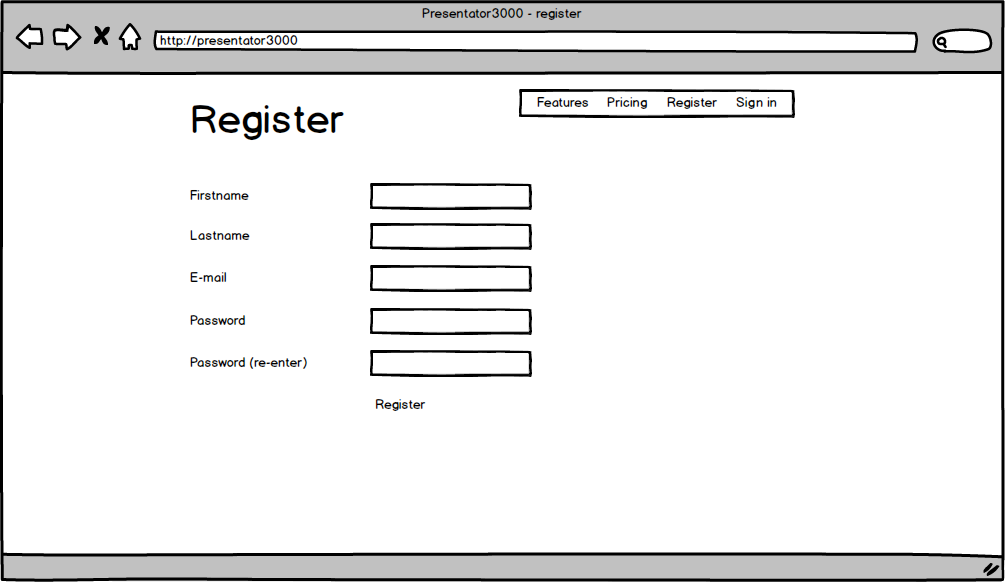
\includegraphics[width=1\textwidth]{images/mockup-register.png}
    \caption{Mockup für Login Screen}
\end{figure}

\section{Login}
\begin{figure}[H]
	\centering
    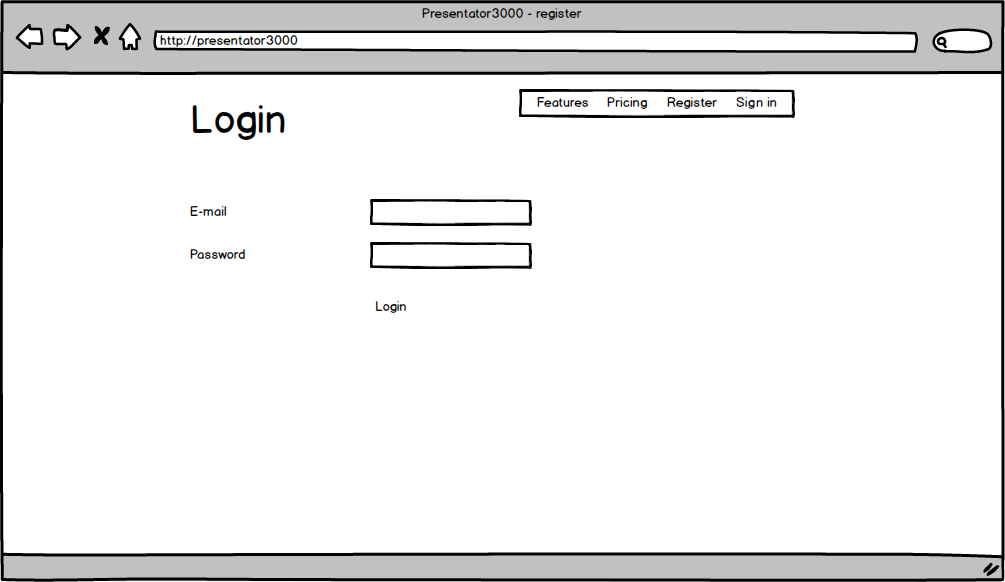
\includegraphics[width=1\textwidth]{images/mockup-login.png}
    \caption{Mockup für Login Screen}
\end{figure}

\section{Präsentationsübersicht}
\begin{figure}[H]
	\centering
    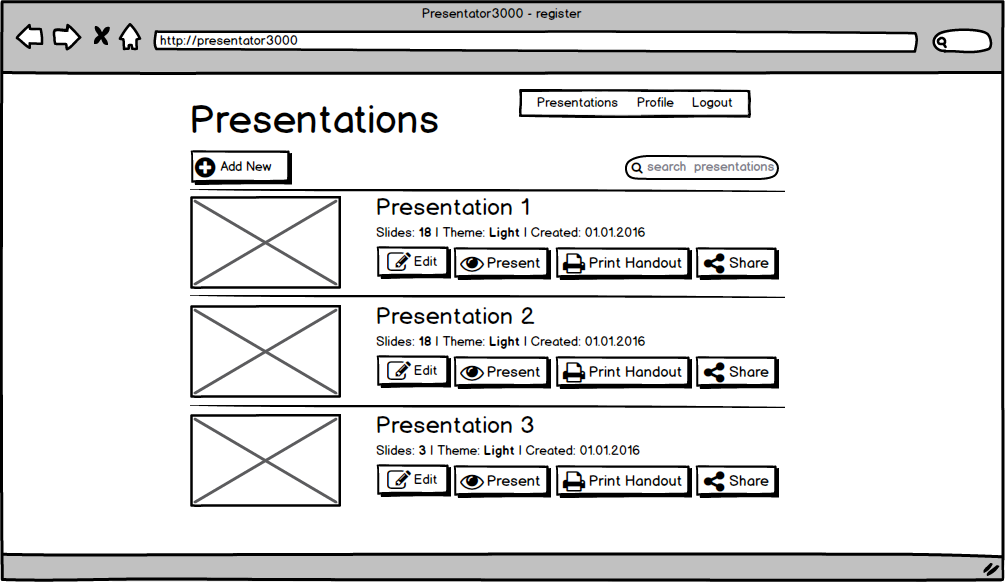
\includegraphics[width=1\textwidth]{images/mockup-presentation-overview.png}
    \caption{Mockup für Login Screen}
\end{figure}

\section{Editoransicht}
\begin{figure}[H]
	\centering
    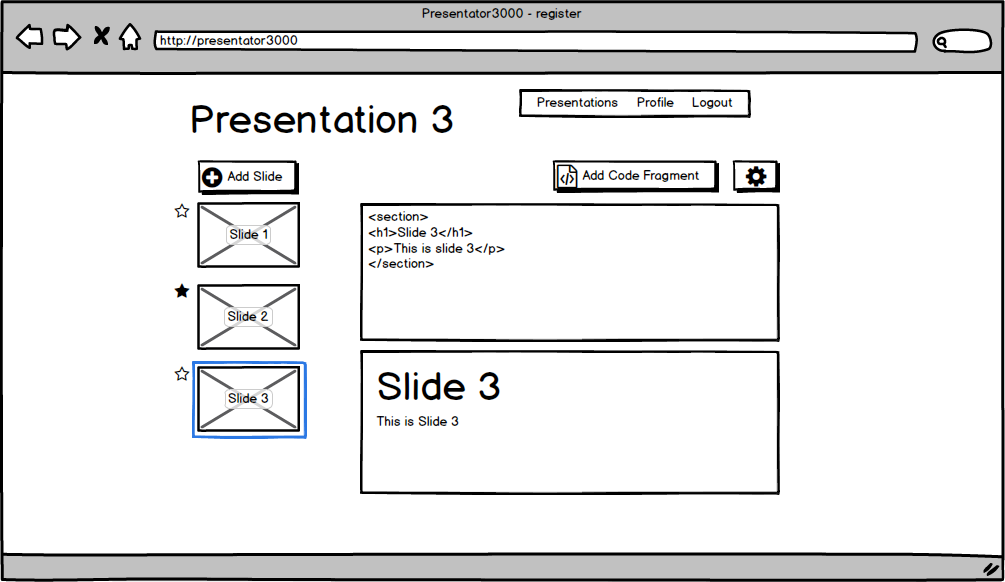
\includegraphics[width=1\textwidth]{images/mockup-presentation-edit.png}
    \caption{Mockup für Login Screen}
\end{figure}

\section{Präsentationseinstellungen}
\begin{figure}[H]
	\centering
    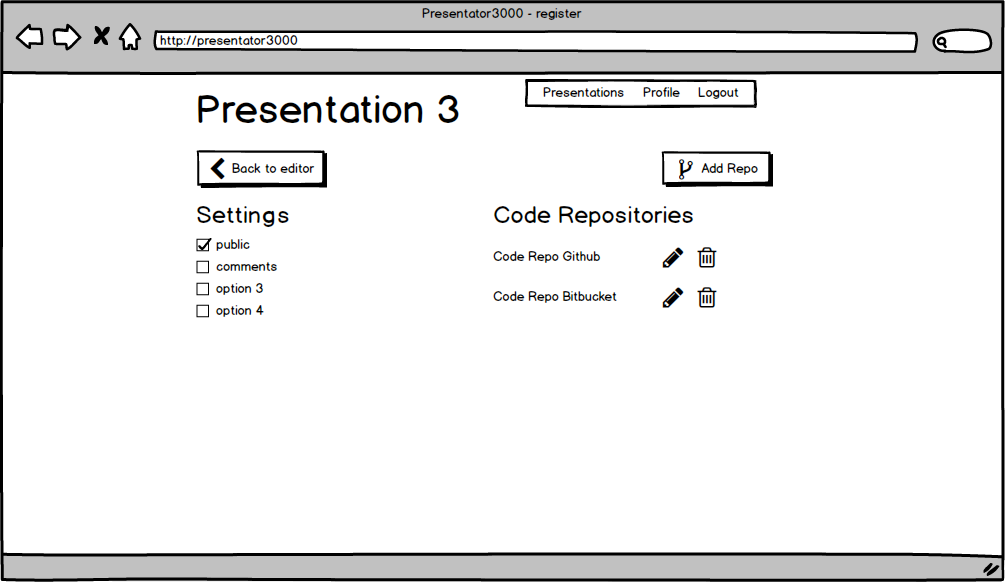
\includegraphics[width=1\textwidth]{images/mockup-presentation-settings-view.png}
    \caption{Mockup für Login Screen}
\end{figure}


\chapter{Dokumentation API}
\label{chap:doc-api}
\section{Grundsatz}
Die ganze Service-Schicht, also das Backend oder auch API genannt, ist eigentlich eine Abstraktion des CRUD-Schemas. CRUD ist ein Akronym und steht für Create, Read, Update und Delete. Dies sind die grundsätzlichen Datenbank-Optionen. Die API erlaubt es, dem Frontend diese Operationen in der Presistenzschicht auszuüben. Für RESTful APIs ist es üblich, die unterschiedlichen HTTP-Methoden, umgangssprachlich auch als HTTP Verbs bezeichnent, zu verwenden. (Beschrieben in RFC 2616, Hypertext Transfer Protocol - HTTP 1.1\footnote{\url{https://www.w3.org/Protocols/rfc2616/rfc2616-sec9.html}}).

Die Zuordnung lautet wie folgt: \\\\
\vspace{0.5cm}
\begin{tabular}{|l|l|p{6cm}|}
\hline
\textbf{CRUD-Opertaion} & \textbf{HTTP-Methode} & \textbf{Bedeutung} \\ \hline	
Create & POST & Eine neue Resource anlegen \\ \hline	
Read & GET & Eine Resource lesen, anschauen \\ \hline	
Update & PUT / PATCH & Eine Resource aktualisieren \\ \hline	
Delete & DELETE & Eine Resource löschen \\ \hline	
\end{tabular}
\vspace{0.3cm}

Als Antworten werden im HTTP Header Statuscodes gesetzt. Auch diese sind im \emph{RFC 2616} beschrieben. Hier findet ebenfalls eine Zuordnung statt:\\\\
\begin{tabular}{|l|l|p{9cm}|}
\hline
\textbf{Code} & \textbf{Bezeichnung} & \textbf{Bedeutung in der API} \\ \hline	
200 &	OK	& Anfrage erfolgreich, Resource im Content (bei GET) oder Änderung erfolgreich, geänderte Resource im Content (bei PUT/PATCH)\\ \hline
201 &	CREATED &	Neue Resource angelegt \\ \hline
204 &	NO CONTENT &	Resource erfolgreich gelöscht \\ \hline
404 &	NOT FOUND	& 	Resource nicht gefunden \\ \hline
422 &	UNPROCESSABLE ENTITY	&	Die Angehängten Daten entsprechen nicht dem erwarteten Format (z.B. wenn Attribute fehlen bei einem POST)\\ \hline
\end{tabular}
\vspace{0.3cm}

\section{Anmerkungen zur Implementation}
Bei der Implementation wurden schliesslich Routen angelegt \emph{service/routes/api.php}, wo beschrieben wird welche URLs akzeptiert werden und delegiert wird, welcher Controller zuständig ist. Wird eine Resource direkt als \emph{Route::resource()} erfasst, findet bereits eine Zuteilung der Methoden zu den entsprechenden HTTP-Verben statt. Ansonsten kann die Methode spezifiziert werden: \emph{Route::get('slides/{id}/comments', 'CommentsController@index');}. Hier wird die Methode \textbf{index} im \textbf{CommentsController} verwendet, falls die URI \emph{api/slides/{slide-id}/comments} aufgerufen wird. In der entsprechenden Methode werden dann \emph{Models} angelegt, aus der Datenbank geholt oder Datensätze gelöscht. Hier bietet Laravel mit Eloquent die entsprechenden Schnittstellen, sodass keine SQL-Queries von Hand geschrieben werden müssen. Wird eine Antwort als JSON zurückgegeben, laufen die Datensätze durch eine weitere Klasse: Ein Transformer. Dieser hat die Aufgabe, die Daten so aufzubereiten, dass das ausgegebene JSON-Objekt korrekt formatiert ist und nur die Daten enthält, welche für das Frontend benötigt werden. So werden hier beispielsweise die PHP-Datumsobjekte vereinfacht und nur ein Date-String zurückgegeben für das Feld \emph{updated_at}. Auch werden hier Links für eingebettete (nested) Resourcen erzeugt. Der Zweck wird später in dieser Dokumentation noch erläutert.

\section{Routen}
In der nachfolgenden Tabelle sind die Routen aufgeführt, welche die API zur Verfügung stellt. Es ist jeweils angegeben, welche HTTP-Methode verwendet werden muss, um auf die Resource mit der entsprechenden Aktion zuzugreifen. In den geschweiften Klammern sind die Parameter angegeben, welche direkt per URI mitgegeben werden. Für die Methoden \textbf{POST} sowie \textbf{PUT} beziehungsweise \textbf{PATCH} muss ein Content mitgegeben werden. Der Content-Typ muss deswegen auf \emph{application/json} gesetzt werden.

\begin{table}[H]
\scriptsize	 
\begin{tabular}{|l|l|l|l|}
\hline
\textbf{Methode} & \textbf{URI} & \textbf{Name} & \textbf{Action} \\ \hline
 GET\&HEAD &  /  & direkt    & web \\ \hline
 GET\&HEAD  & /api  & direkt    & \\ \hline
 POST & api/attachements & attachements.store & App\textbackslash{}Http\textbackslash{}Controllers\textbackslash{}AttachementsController\@store  \\ \hline
 GET\&HEAD & api/attachements  & attachements.index & App\textbackslash{}Http\textbackslash{}Controllers\textbackslash{}AttachementsController\@index  \\ \hline
 DELETE & api/attachements/\{attachement\} & attachements.destroy & App\textbackslash{}Http\textbackslash{}Controllers\textbackslash{}AttachementsController\@destroy  \\ \hline
  PUT\&PATCH  & api/attachements/\{attachement\} & attachements.update & App\textbackslash{}Http\textbackslash{}Controllers\textbackslash{}AttachementsController\@update  \\ \hline
 GET\&HEAD & api/attachements/\{attachement\} & attachements.show & App\textbackslash{}Http\textbackslash{}Controllers\textbackslash{}AttachementsController\@show  \\ \hline
 POST & api/channels  & channels.store  & App\textbackslash{}Http\textbackslash{}Controllers\textbackslash{}ChannelsController\@store  \\ \hline
 GET\&HEAD & api/channels  & channels.index  & App\textbackslash{}Http\textbackslash{}Controllers\textbackslash{}ChannelsController\@index  \\ \hline
 DELETE & api/channels/\{channel\}  & channels.destroy & App\textbackslash{}Http\textbackslash{}Controllers\textbackslash{}ChannelsController\@destroy  \\ \hline
  PUT\&PATCH  & api/channels/\{channel\}  & channels.update  & App\textbackslash{}Http\textbackslash{}Controllers\textbackslash{}ChannelsController\@update  \\ \hline
 GET\&HEAD & api/channels/\{channel\}  & channels.show  & App\textbackslash{}Http\textbackslash{}Controllers\textbackslash{}ChannelsController\@show  \\ \hline
 POST & api/channels/\{cid\}/presentations/\{pid\} & add_presentation_to_channel & App\textbackslash{}Http\textbackslash{}Controllers\textbackslash{}ChannelsController\@add  \\ \hline
 GET\&HEAD & api/channels/\{id\}/presentations & channel_presentations & App\textbackslash{}Http\textbackslash{}Controllers\textbackslash{}PresentationsController\@index  \\ \hline
 GET\&HEAD & api/comments  & comments.index  & App\textbackslash{}Http\textbackslash{}Controllers\textbackslash{}CommentsController\@index  \\ \hline
 POST & api/comments  & comments.store  & App\textbackslash{}Http\textbackslash{}Controllers\textbackslash{}CommentsController\@store  \\ \hline
 GET\&HEAD & api/comments/\{comment\}  & comments.show  & App\textbackslash{}Http\textbackslash{}Controllers\textbackslash{}CommentsController\@show  \\ \hline
  PUT\&PATCH  & api/comments/\{comment\}  & comments.update  & App\textbackslash{}Http\textbackslash{}Controllers\textbackslash{}CommentsController\@update  \\ \hline
 DELETE & api/comments/\{comment\}  & comments.destroy & App\textbackslash{}Http\textbackslash{}Controllers\textbackslash{}CommentsController\@destroy  \\ \hline
 POST & api/presentations  & presentations.store & App\textbackslash{}Http\textbackslash{}Controllers\textbackslash{}PresentationsController\@store  \\ \hline
 GET\&HEAD & api/presentations  & presentations.index & App\textbackslash{}Http\textbackslash{}Controllers\textbackslash{}PresentationsController\@index  \\ \hline
 POST & api/presentations/\{id\}/attachements & add_attachement_to_presentation & App\textbackslash{}Http\textbackslash{}Controllers\textbackslash{}AttachementsController\@store  \\ \hline
 GET\&HEAD & api/presentations/\{id\}/attachements & presentation_attachements & App\textbackslash{}Http\textbackslash{}Controllers\textbackslash{}AttachementsController\@index  \\ \hline
 POST & api/presentations/\{id\}/slides & add_slide_to_presentation & App\textbackslash{}Http\textbackslash{}Controllers\textbackslash{}SlidesController\@store  \\ \hline
 GET\&HEAD & api/presentations/\{id\}/slides & presentation_slides & App\textbackslash{}Http\textbackslash{}Controllers\textbackslash{}SlidesController\@index  \\ \hline
  PUT\&PATCH  & api/presentations/\{presentation\} & presentations.update & App\textbackslash{}Http\textbackslash{}Controllers\textbackslash{}PresentationsController\@update  \\ \hline
 DELETE & api/presentations/\{presentation\} & presentations.destroy & App\textbackslash{}Http\textbackslash{}Controllers\textbackslash{}PresentationsController\@destroy  \\ \hline
 GET\&HEAD & api/presentations/\{presentation\} & presentations.show & App\textbackslash{}Http\textbackslash{}Controllers\textbackslash{}PresentationsController\@show  \\ \hline
 GET\&HEAD & api/slides  & slides.index  & App\textbackslash{}Http\textbackslash{}Controllers\textbackslash{}SlidesController\@index  \\ \hline
 POST & api/slides  & slides.store  & App\textbackslash{}Http\textbackslash{}Controllers\textbackslash{}SlidesController\@store  \\ \hline
 GET\&HEAD & api/slides/\{id\}/comments & slide_comments  & App\textbackslash{}Http\textbackslash{}Controllers\textbackslash{}CommentsController\@index  \\ \hline
 POST & api/slides/\{id\}/comments & add_comment_to_slide & App\textbackslash{}Http\textbackslash{}Controllers\textbackslash{}CommentsController\@store  \\ \hline
  PUT\&PATCH  & api/slides/\{slide\}  & slides.update  & App\textbackslash{}Http\textbackslash{}Controllers\textbackslash{}SlidesController\@update  \\ \hline
 DELETE & api/slides/\{slide\}  & slides.destroy  & App\textbackslash{}Http\textbackslash{}Controllers\textbackslash{}SlidesController\@destroy  \\ \hline
 GET\&HEAD & api/slides/\{slide\}  & slides.show  & App\textbackslash{}Http\textbackslash{}Controllers\textbackslash{}SlidesController\@show  \\ \hline
 POST & api/templates  & templates.store  & App\textbackslash{}Http\textbackslash{}Controllers\textbackslash{}TemplatesController\@store  \\ \hline
 GET\&HEAD & api/templates  & templates.index  & App\textbackslash{}Http\textbackslash{}Controllers\textbackslash{}TemplatesController\@index  \\ \hline
 DELETE & api/templates/\{template\} & templates.destroy & App\textbackslash{}Http\textbackslash{}Controllers\textbackslash{}TemplatesController\@destroy  \\ \hline
  PUT\&PATCH  & api/templates/\{template\} & templates.update & App\textbackslash{}Http\textbackslash{}Controllers\textbackslash{}TemplatesController\@update  \\ \hline
 GET\&HEAD & api/templates/\{template\} & templates.show  & App\textbackslash{}Http\textbackslash{}Controllers\textbackslash{}TemplatesController\@show  \\ \hline
 POST & api/user  & user.store  & App\textbackslash{}Http\textbackslash{}Controllers\textbackslash{}UserController\@store  \\ \hline
 GET\&HEAD & api/user  & user.index  & App\textbackslash{}Http\textbackslash{}Controllers\textbackslash{}UserController\@index  \\ \hline
 GET\&HEAD & api/user/create  & user.create  & App\textbackslash{}Http\textbackslash{}Controllers\textbackslash{}UserController\@create  \\ \hline
 DELETE & api/user/\{user\}  & user.destroy  & App\textbackslash{}Http\textbackslash{}Controllers\textbackslash{}UserController\@destroy  \\ \hline
 GET\&HEAD & api/user/\{user\}  & user.show  & App\textbackslash{}Http\textbackslash{}Controllers\textbackslash{}UserController\@show  \\ \hline
  PUT\&PATCH  & api/user/\{user\}  & user.update  & App\textbackslash{}Http\textbackslash{}Controllers\textbackslash{}UserController\@update  \\ \hline
 GET\&HEAD & api/user/\{user\}/edit  & user.edit  & App\textbackslash{}Http\textbackslash{}Controllers\textbackslash{}UserController\@edit  \\ \hline
 \end{tabular}
\end{table}
 
\section{Datenaustausch}
 Die Datentransfers zum Frontend werden mittels der JavaScript Object Notation (JSON) realisiert. JSON ist ein kompaktes Datenformat, welches von der Programmiersprache unabhängig ist. Es ist der quasi-Standard für RESTful APIs. Da ursprünglich aus dem JavaScript stammt, benötigt Javascript keinen Parser, was zu einem Performance Gewinn führt. 
 
\subsection{Beispiel}
Zur Verdeutlichung wird hier nachfolgend ein kleines Beispiel aufgezeigt: Hier wird vom Frontend aus eine Anfrage für ein "Attachment" gesendet, also ein HTTP-Request vom Typ "GET" an die URI \emph{http://presentator3000.app/api/attachements/2}. Im Content der Response ist folgendes JSON-Objekt zu finden: 
\begin{lstlisting}[caption=JSON als Antwort auf einen GET-Request]
{
  "id" : 2,
  "filename" : "eb793ea81f9c9a.xpm",
  "presentation" : "http://presentator3000.app/api/presentations/14",
  "updated_at" : "2016-12-27 11:02:19"
}
\end{lstlisting}

Diese Informationen können nun vom Frontend verarbeitet werden und dem User im Browser angezeigt werden. Um das Beispiel zu erweitern, ist nachfolgenden das JSON Objekt aufgeführt, welches gesandt werden muss, um eine neue Slide anzulegen. Hier wird ein POST-Request verschickt an \emph{presentator3000.app/api/presentation/12/slides}. Dies bedeutet, dass eine neue Slide-Resource bei der Präsentation mit der ID \emph{12} angelegt werden soll:

\begin{lstlisting}[caption=POST Request um eine neue Slide anzulegen]
{
  "content" : "<h1>Eine neue Slide</h1><p>Hier ist eine neue Slide</p>",
  "shared" : false
}
\end{lstlisting}

Dies wird von der API, also dem Backend verarbeitet. Zuerst wird überprüft, ob die nötigen Informationen vorhanden sind. Bei einer Slide ist dies nur das Attribut \emph{content}. Das Attribut \emph{shared} ist optional. Wird es nicht mitgegeben, greift der default Wert und der ist in diesem Fall \textbf{false}. Wird ein zwingender (required) Wert nicht mitgeliefert, antwortet die API mit einem Fehler. Hierzu wird eine HTTP-Response mit dem entsprechenden Statuscode abgesetzt. In diesem Fall ist dies der Code \emph{422}, welcher für \emph{HTTP UNPROCESSABLE ENTITY} steht. Ist alles wie erwartet vorhanden, wird ein neues PHP-Objekt erzeugt und persistiert. Beim Eintrag in die Datenbank wird dabei eine ID generiert. Die ID wird unter Umständen im Frontend für die Weiterverarbeitung benötigt. Deshalb wurde der Service so umgesetzt, dass auch bei jedem POST, PUT oder PATCH ein Body mitgegeben wird, welcher gleich das erzeugte Objekt (inklusive ID) enthält. Diese Response sähe im obigen Beispiel wie folgt aus:

\begin{lstlisting}[caption=HTTP Response für eine neu anglegte Slide]
{
  "data": {
    "id": 21,
    "content": "<h1>Eine neue Slide</h1><p>Hier ist eine neue Slide</p>",
    "shared": false,
    "comments": "http://presentator3000.app/api/slides/21/comments",
    "updated_at": "2016-12-27 08:02:10"
  },
  "message": "Slide successfully created."
}
\end{lstlisting}
Der HTTP-Statuscode im Erfolgsfall lautet \emph{201 - CREATED}. Wie ersichtlich ist, beinhaltet die Antwort ein JSON Objekt mit zwei Attributen erster Ebene. Einerseits die Daten (\emph{data}) und andererseits die Meldung (\emph{message}). Im Daten-Attribut ist ein weiteres Objekt enthalten, die erstellte Slide. Hier wird nicht nur die ID zurückgegeben, sondern auch einen Link auf genestete Attribute, hier beispielsweise die Kommentare (\emph{Comments}). Statt diese direkt auszugeben, was zu einer Performance-Einbusse führen könnte, wird lediglich der URI mitgegeben. Das Frontend kann dann direkt auf diese Resource zugreifen. Dieses Prinzip schneidet das Programmier-Paradigma \textbf{HATEOAS}\footnote{HATEOAS steht für Hypermedia As The Engine Of Application State und ist eine Erweiterung der klassischen REST Architektur beziehungsweise die höchste Form der Abstraktion zwischen Frontend und Backend. (\url{https://en.wikipedia.org/wiki/HATEOAS})} an. Natürlich ist dies bloss der Anfang. Man könnte weiter auch URLs für die verschiedenen CRUD Operationen aufführen, wie beispielsweise die Links für Update oder Delete einer Resource. 
\chapter{Entwicklung und Testing}
\label{chap:testing}

\section{Entwicklung des Frontends}
Hier wurde der Node Package Manager (\emph{npm}) verwendet, um die Dependencies zu beziehen. Mit Webpack wurde das Javascript und die vue-Template Dateien in eine Javascript-Datei kompiliert. Webpack bringt mit dem Befehl \emph{npm run dev} auch gleich einen kleinen Webserver mit, welcher den Vorteil bringt, dass man nicht nach jeder Änderung den Code neu kompilieren muss, sonder dieser laufend im Browser aktualisiert (injected) wird.

\section{Entwicklung des Backends}
Für die Entwicklung der API wurde, wie bereits erwähnt, Laravel eingesetzt. Für den lokalen Betrieb wird eine Virtuelle Maschine empfohlen. Hier wurde Vagrant mit einem Homestead Container verwendet. Als Datenbank kam das mit dem Homestead mitgelieferte mySQL zum Einsatz.

Die Virtuelle Maschine kann durch den lokal eingerichteten Pfad \url{http://presentator3000.app/api/} angesteuert werden.

Um das Zusammenspiel der API mit dem Frontend zu testen, wurde auf einem Webserver eine Stage aufgesetzt. Die Zugänge lauten wie folgt:

\begin{itemize}
	\item \textbf{Frontend:} \url{http://3000.uahnn.com/}
	\item \textbf{Backend:} \url{http://presentator3000.uahnn.com/api/}
\end{itemize}

Zudem wurden bei der API 2 Routen angelegt, eine für die URL direkt und eine für \emph{/api} mit Testcontent, um die Funktionalität einfach zu überprüfen (läuft das System noch).

Um die Datenbank zu testen, wurden mit Hilfe von Seedern Demo-Daten abgefüllt. Die Datenbank-Tabellen wurde nicht direkt mit SQL Queries angelegt, sondern durch Migrations (in Laravel). Dies sind PHP-Container, welche durch Methoden die jeweiligen Tabellen und Felder anlegen. Dies ermöglichte eine laufende Anpassung des Datenbank-Modells. Bei jeder Anpassung konnten so die Demodaten durch die Seeder erneut erzeugt werden. Somit hat man zu jeder Zeit passende Demo-Daten. 

\section{Testing der API}
Um die Entwicklung von API und Frontend unabhängig von einander voranzutreiben, mussten die API-Calls separat getestet werden. Hier wurde das Tool \emph{Postman} verwendet. Es handelt sich hierbei um eine kostenlose Browsererweiterung für Google Chrome. Hier können jegliche HTTP-Requests erstellt, gespeichert und abgesetzt werden. Dies erlaubte auch das Testen von Resourcen und Routes, welche im Frontend noch nicht implementiert waren. So konnte die Struktur der JSON Objekte laufen überprüft werden, und falls sie ungeeignet waren, wurden sie direkt wieder angepasst. Postman erlaubt ausserdem das Exportieren von Collections, um diese anderen Usern zur Verfügung zu stellen. Die verwendete Collection liegt dieser Dokumentation bei.

\begin{figure}[H]
	\centering
    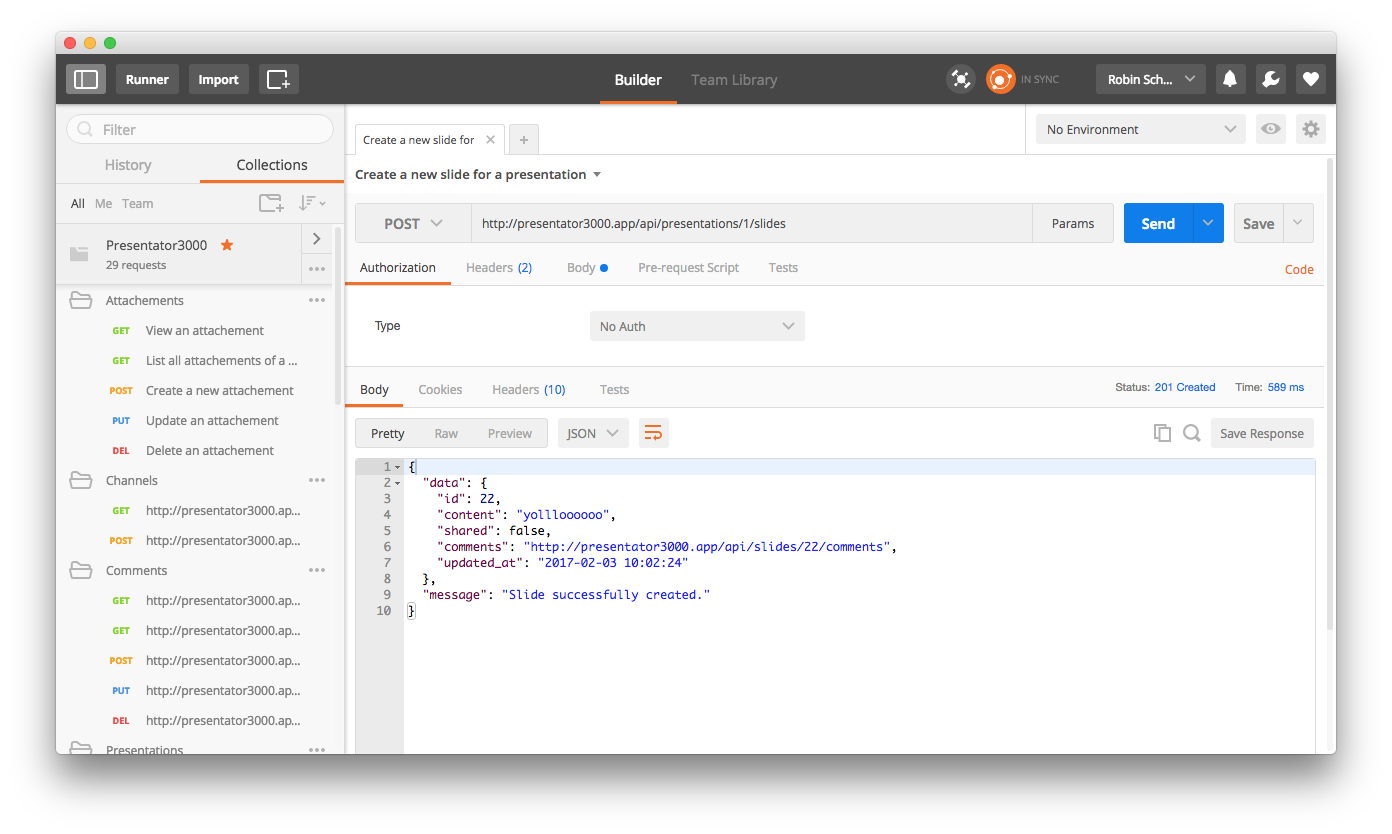
\includegraphics[width=1\textwidth]{images/printscreen-postman.png}
    \caption{Printscreen der Postman Applikation}
\end{figure}
\chapter{Fazit}
\label{chap:fazit}

\section{Gelerntes}
Wir konnten uns in der kurzen Zeit viel Wissen über aktuellste Frontend- und Backend-Technologien aneignen. Dies erlaubte die Entwicklung einer sehr weit ausgebauten API. Das Konzept wurde grundsätzlich getestet und die Anforderung für ein fertiges Produkt wurden definiert. Durch das Projekt sind grundlegende Entscheide bereits gefällt und getestet worden. 

Die Absprachen im Team waren zu beginn des Projekts sehr gut verlaufen. Beide Teammitglieder wussten genau, was sie wie umzusetzen haben. So konnten die Anforderungen nach Routen bei Frontend direkt vom anderen Teammitglied im Backend umgesetzt werden. Auch die Absprachen mit dem Dozenten verliefen sehr konstruktiv. Gegen Ende des Projekts war jedoch spürbar, dass die Konzentration nachgelassen hatte. Leider wurde der Kontakt zum Betreuer nicht mehr intensiv gepflegt, was wiederum zu Missverständnissen führte innerhalb des Teams. Positiv hervorzuheben ist aber der Einsatzwille, welcher sich auch in den 4 durchgeführten Hackathons (Samstags oder Sonntags) äusserte, welche während des Projekts durchgeführt wurden. Durch die Anwesenheit von beiden konnte das Teamwork gefördert werden und Absprachen konnten direkt mündlich geführt werden. Leider konnte diese Mentalität nicht bis zum Schluss weitergezogen werden, auch wegen der Abwesenheit von Herrn Schmid.

In künftigen Projekten muss der Kommunikation intern und extern mehr Bedeutung beigemessen werden. Hier müssten im Projektplaungstool (es wurde \emph{trello} verwendet) nicht nur Tasks für Code und Doku sondern auch Kommunikationsaufgaben erfasst werden.

\section{Ausblick}
Eine künfige Thesis (oder auch Projekt 1/2) kann auf der geleisteten Arbeit basieren. Das Datenbank-Konzept und die Kommunikation zwischen Frontend und Backend sind erprobt. Die eingesetzten Technologien haben sich bewährt. Es ist jedoch anzumerken, dass alle Technologien eine gewisse Einarbeitungszeit haben. Für ein Proof-of-Concept waren die eingesetzten Frameworks unter Umständen bereits zu massiv. Das Konzept bietet viele Erweitungsmöglichkeiten. Es konnten im Rahmen der Projektarbeit auch noch nicht alle Funktionalitäten vollständig umgesetzt werden. Eine weiterführende Arbeit kann hier ansetzen und die erstellten Dokumentationen und Codelines verwenden.


\end{document}
